\documentclass[]{article}

\usepackage{amsmath}
\usepackage{amsfonts}
\usepackage{hyperref, bookmark}
\bibliographystyle{IEEEtran}

\usepackage{graphicx}
\graphicspath{ {./Fig/} }

% \setlength{\parindent}{0cm}
\usepackage[margin=1in]{geometry}

% \bibliography{reference}
\setlength{\parskip}{1em}

%opening
\title{Boletín Laboratorio 2}
\author{Ignacio Osorio}

\begin{document}

\maketitle

\begin{abstract}

En este laboratorio se trabajó en búsquedas de texto del tipo \emph{pattern matching}. Se implemento un \emph{Suffix Array} \cite{SuffixArray} y una búsqueda lineal para poder comparar los comportamientos de ambas formas de abordar el problema. Los datos de prueba fueron de una base de datos de texto que se puede encontrar en \emph{Pizza\&Chili Corpus} \cite{data}, específicamente el archivo de 50 mbs de texto en inglés ($\sim$58M de caracteres). Se analizara también el tiempo de preprocesamiento necesario para el \emph{Suffix Array} en función del tamaño del texto ingresado.

\end{abstract}

\section{Ejercicio 1}
Los algoritmos fueron implementados en C++ y probados en un computador personal. Las especificaciones del computador se pueden ver en la tabla \ref{tab:spec}. Todos los códigos generados para este laboratorio se encuentran adjuntos a este documento.

\begin{table}[]
	\centering
	\caption{Especificaciones del computador personal.}
	\label{tab:spec}
	\begin{tabular}{|c|c|c|}
		\hline
		CPU 					& RAM 			& SO 	 				\\ \hline
		Intel Core i7-7700HQ    & 16 GB        	& Windows 10 Home        \\ \hline
	\end{tabular}
\end{table}


\section{Ejercicio 2}

Para todas las pruebas se utilizó el mismo texto, el cual se encuentra en inglés.

El \emph{Suffix Array} y la búsqueda por fuerza bruta fueron evaluados comparativamente a través de tres tipos de pruebas. 

En la figura \ref{fig}, subplot \textbf{b)} se observa los tiempos promedio para realizar búsquedas usando un \emph{Suffix Array} y fuerza bruta. Variando en el tamaño del texto de entrada utilizado y calculando el promedio de 20 muestras con distintos tamaños de patrones.

Cabe recalcar que los órdenes de magnitudes son muy distintos entre las mediciones de la estructura y el algoritmo, es por esto que se separaron en distintos ejes y (a la izquierda estarán los tiempos del \emph{Suffix Array} y a la derecha los de fuerza bruta). 

En la figura \ref{fig}, subplot \textbf{c)} se compara los tiempos de búsqueda utilizando el texto completo y variando tamaños del patrón. Se generaron patrones aleatorios para cada búsqueda, sin repetirlos entre la estructura y el algoritmo.

En la figura \ref{fig}, subplot \textbf{d)} se utilizaron las 10 palabras más comunes del inglés según wikipedia \cite{common}.

Una cuarta prueba se realizó para medir el tiempo de construcción de la estructura de dato \emph{Suffix Array}, esto se hizo comparativo al tamaño del texto y se puede observar en la figura \ref{fig}, subplot \textbf{a)}.

Todos los patrones aleatorios fueron extraídos del mismo texto de prueba, asegurando que ninguno de ellos contuviera el carácter que representa el fin de línea $'\setminus n'$.


\begin{figure}[tb]
	\centering
	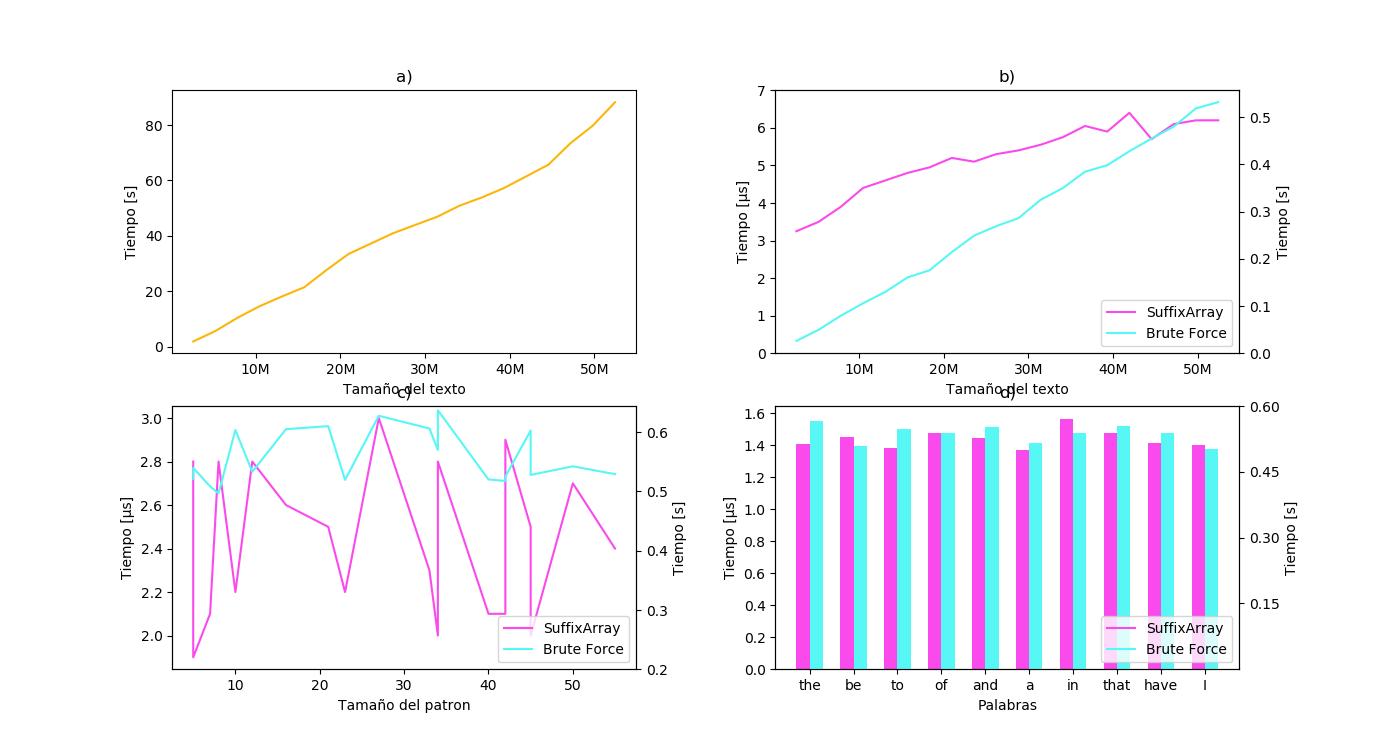
\includegraphics[width=1\textwidth]{fig}
	\caption{\textbf{a)} Tiempo de preprocesamiento para \emph{Suffix Array} vs el tamaño del texto, \textbf{b)} comparación de tiempos de búsqueda usando el SA (en [$\mu$s]) y fuerza bruta (en [s]) con patrones aleatorios vs tamaño del texto, \textbf{c)} búsqueda usando el SA (en [$\mu$s]) y fuerza bruta (en [s]) para un texto de $\sim$58M de caracteres vs tamaño de patrones aleatorios y \textbf{d)} búsqueda de las 10 palabras más comunes del inglés usando el SA (en [$\mu$s]) y fuerza bruta (en [s]).}
	\label{fig}
\end{figure}


\subsection{Análisis}

Para los análisis se denotará $n$ como el largo del texto y $m$ el largo del patrón.

Para el \emph{Suffix Array} la complejidad temporal de la construcción dependerá del algoritmo de ordenamiento utilizado y la complejidad de las comparaciones. Crear el arreglo de índices tendrá orden $O(n)$ y ordenar este arreglo (usando un algoritmo basado en comparaciones) será $O(n*log(n))$ comparaciones. Donde las comparaciones serán en base a los sub-strings que parten desde dicho índice, esto se realiza en $O(n)$ para el peor caso. Por lo que la complejidad temporal de la construcción de esta estructura de datos será $O(n^{2}*log(n))$. 

La complejidad espacial dependerá de $n$ y del alfabeto $\Sigma$. Puesto que cada carácter utilizaría $log_{2}(|\Sigma|)$ bits para su representación y el texto de entrada tendrá $n$ caracteres, podemos calcular que el espacio necesario para representar nuestra estructura de datos correspondería a guardar el texto $O(n*log_{2}(|\Sigma|))$ y guardar el arreglo de índices que corresponde a $O(n*log_{2}(n))$. Si suponemos que nuestro texto tendrá un largo considerablemente mayor que el cardinal de nuestro alfabeto ($n<<|\Sigma|$), podemos asegurar que la complejidad espacial es $O(n*log_{2}(n))$.

Para la búsqueda, la complejidad temporal se descompone en realizar dos búsquedas binarias sobre nuestro arreglo de índices, multiplicado por la complejidad de comparar los strings. Suponiendo que nuestro patrón de búsqueda es considerablemente mayor a nuestro texto ($m<<n$), podemos asegurar que la complejidad del peor caso será $O(m*log_{2}(n))$. La componente logarítmica viene de la búsqueda binaria, mientras que la componente $m$ viene de la complejidad de las comparaciones de los strings.

\section{Conclusiones}

Al no utilizar texto patológico como entrada, la componente cuadrática de la construcción del \emph{Suffix Array} pareciera no encontrarse en la gráfica \ref{fig} \textbf{a)}, sin embargo se observa que cuando el tamaño del texto aumenta demasiado, los tiempos empiezan a funcionar ligeramente cuadrático. Esto se puede deber a que entre mayor sea la base de dato, mayores serán los largos en común entre sufijos, lo que influirá en que las comparaciones deban iterar sobre mas caracteres para poder identificar la precedencia lexicográfica.

A partir de esto mismo, se puede ver que un texto patológico para la estructura sería una que contenga el mismo caracter repetido $n$ veces. Por otro lado, si suponemos texto con caracteres al azar con una distribución gaussiana sobre el alfabeto, se podría concluir que entre menor sea $|\Sigma|$ la construcción de la estructura será más lenta. Esto puesto que la cantidad de palabras distintas que podemos construir con un alfabeto $\Sigma$ con $n$ caracteres distintos, dependerá de dicho cardinal.

El uso de la estructura de datos para la búsqueda de patrones se comporta excepcionalmente mejor que la fuerza bruta. Aproximadamente en el orden de $10^{7}$. 

Se puede observar su comportamiento logarítmico de la estructura de dato frente al tamaño de datos en la figura \ref{fig} \textbf{b)} y el comportamiento lineal de la búsqueda por fuerza bruta.

Se puede ver en la figura \ref{fig} \textbf{c)} que habrá casos donde el largo de comparaciones efectivas promedio de los patrones será mayor y esto hará que se comporte más lenta la búsqueda. Teniendo el largo del patrón como una cota superior. En practica, dependerá de las comparaciones de caracteres realizadas más que sobre el largo del patrón.

En la búsqueda utilizando las palabras más frecuentes se observó que los tiempos necesarios usando la estructura eran demasiado bajos. Esto como prueba con datos y patrones reales.

Finalmente se puede concluir que se debe tener presente el \emph{trade-off} de usar esta estructura de datos frente a una solución logarítmica al problema de \emph{pattern matching}, esto puesto que la construcción de la estructura \emph{Suffix Array} fue considerablemente lenta para datos de entrada masivos, demorándose más de un minuto. Se deberá tener atención para casos donde el número de consultas sobre nuestra estructura hagan practico su uso por sobre una solución algorítmica.

\pdfbookmark{Bibliografía}{bibliografia}
\bibliography{reference}

\end{document}
